\chapter{Detailed Existing study}

\section*{Introduction}
In this chapter, we will explain various concepts that are crucial for the subsequent sections of this report. We will also do a thorough detailed study of the current environment the existing architecture and the deployment process.

\section{Cloud Computing}
\paragraph*{Definition:}
Cloud computing is the on-demand availability of computer system resources, especially data storage and computing power, without direct active management by the user. A simple way to describe the Cloud is its multiple data centers available to many users over the Internet.
\par
\noindent
Cloud computing services are offered by various providers, with Amazon Web Services, Microsoft Azure, and Google Cloud Platform being some of the major players in the field.
\subsection*{Comparative study between cloud providers}
So it makes sense to compare the three major cloud providers to see which one is the best for our project.
\subsubsection*{strengths of the three major cloud providers \cite{webArticle1}}
\begin{itemize}
    \item \textbf{Amazon Web Services (AWS):} AWS has had almost a 7-year head-start and vastly more offerings at present than other competitors. With that head start, the available talent pool is larger, meaning that more people know AWS.
    \item \textbf{Microsoft Azure:} Azure provides a pretty compelling transition path to the cloud, also Microsoft has a large number of enterprise customers, and many of them are already using Microsoft products. This makes it easier for them to use Azure.
    \item \textbf{Google Cloud Platform (GCP):} Google just happens to originated one of the most popular container orchestration systems, that being Kubernetes. and with that, it has been able to leverage that reputation to attract customers to its cloud platform.
\end{itemize}
\subsubsection*{Weaknesses of the three major cloud providers \cite{webArticle1}}
\begin{itemize}
    \item \textbf{Amazon Web Services (AWS):} With its vast growth Amazon (the company that owns AWS) has become a direct rival to many retailers, and that has led to some customers looking for alternatives.
    \item \textbf{Microsoft Azure:} For the past decade or so, open-source software has found great acceptance, both on-prem and in the cloud, largely due to organizations seeking alternatives to commercial software vendors like Microsoft.
    \item \textbf{Google Cloud Platform (GCP):} Google has a reputation for killing off products that don't meet its expectations, and that has led to some customers being wary of using Google Cloud Platform.
\end{itemize}
\subsection*{Verdict}
since this project is about transitioning to the cloud, and the fact that the company Adactim has a golden partnership with Microsoft, we will be using Microsoft Azure as our cloud provider.


\section{Cloud Computing Services}
\paragraph*{Definition:} Cloud computing services are a broad set of services that are delivered over the internet. These services are divided into three main categories: Infrastructure as a Service (IaaS), Platform as a Service (PaaS), and Software as a Service (SaaS).
\subsection*{IaaS}
\noindent
\textbf{Definition:} IaaS provides virtualized computing resources that require the developer to manage the infrastructure, including the network, servers, and operating systems. and with this comes great flexibility and scalability.
\noindent \\
\textbf{Offered Services:} Azure offers a wide range of IaaS services, including virtual machines, storage, and networking. With this, we can simulate the on-premises infrastructure in the cloud with minimal changes.
\subsection*{PaaS}
\noindent
\textbf{Definition:} PaaS provides a platform allowing developers to build, run, and manage applications without the complexity of building and maintaining the infrastructure. This allows developers to focus on the application itself.
\noindent \\
\textbf{Offered Services:} Some of the PaaS services offered by Azure include Azure App Service and Azure Functions. and these services have built-in deployment strategies that can be selected.
\subsection*{SaaS}
\noindent
\textbf{Definition:} SaaS is a software distribution model in which applications are hosted by a third-party provider so developers don't have to install, maintain, or update the software.
\noindent \\
\textbf{Offered Services:} Azure offers a wide range of SaaS services, including Office 365, Dynamics 365, and many more. Unfortunately, these services are not relevant to us since we cannot use them to host our application.
\subsection*{Verdict}
After this brief overview of the cloud computing services, we can conclude that the IaaS and PaaS services are the most relevant to us, so I will implement the deployment plan using both of them and choose the most suitable one.
\section{Infrastructure Study}
The company is currently using the baseline web application architecture provided by Microsoft\cite{webArticle6}.
This figure \ref{fig:gloabal_architecture} presents the global architecture of the application.

\begin{figure}[htpb]
    \centering
    \frame{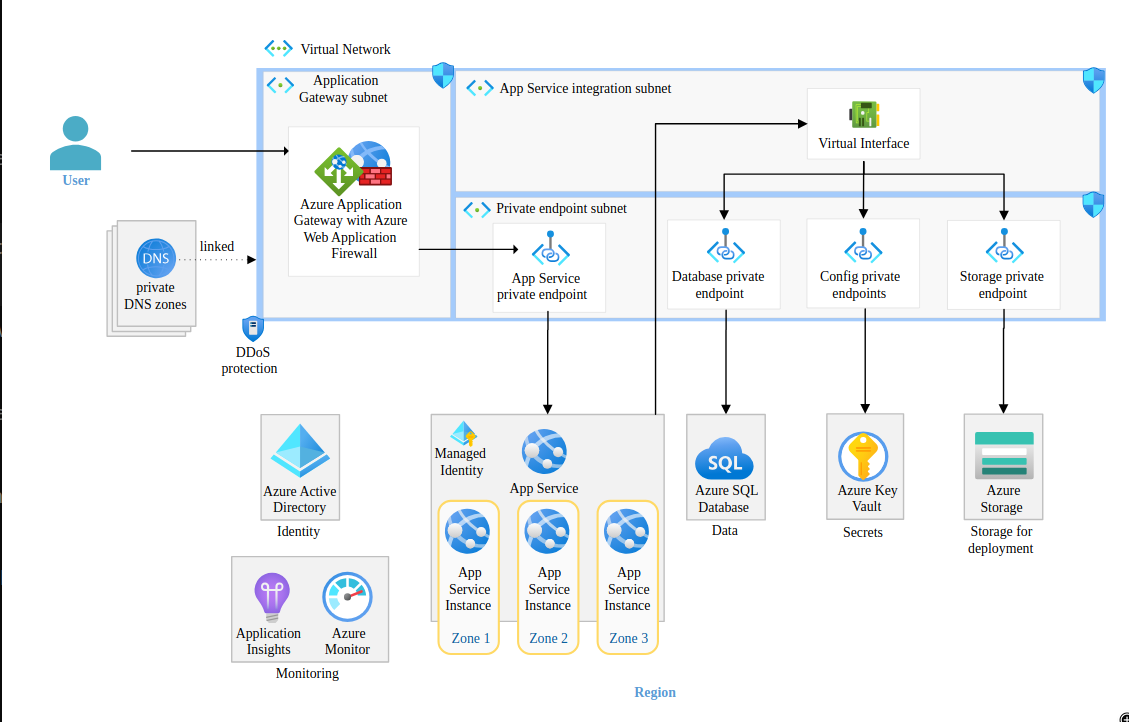
\includegraphics[width=0.5\columnwidth]{global_architecture.png}}
    \caption{gloabal architecture}
    \label{fig:gloabal_architecture}
\end{figure}

\noindent \textbf{Description:} The architecture exposes a public endpoint via Azure Application Gateway with Web Application Firewall. The App Service application uses virtual network integration to securely communicate to Azure PaaS services such as Azure Key Vault and Azure SQL Database.

\subsection*{Componants of the architecture}
\begin{itemize}
    \item \textbf{Virtual Network:} This is the fundamental building block for your private network in Azure. It provides isolation and protection for your resources.
    \item \textbf{App Service:} This service is used to host the web application. It provides a fully managed platform for building, deploying, and scaling web apps.
    \item \textbf{Azure SQL Database:} This service is used to store the application data. It provides a fully managed relational database with built-in high availability and security.
    \item \textbf{Azure Key Vault:} This service is used to store and manage application secrets. It provides a secure and centralized storage for application secrets.
    \item \textbf{Azure Application Gateway:} This service is used to protect the web application from common web vulnerabilities. It provides a web application firewall and other security features.
    \item \textbf{Azure Monitor:} This service is used to monitor the health of the web application. It provides logging and application telemetry to monitor the health of the application.
    \item \textbf{Azure DevOps:} This service is used to automate the deployment of the web application. It provides a set of tools for building, testing, and deploying applications.
    \item \textbf{Virtual Interface:} This service is used to connect the web application to the virtual network. It provides a secure and private connection to the web application.
    \item \textbf{Application Insights:} This service is used to monitor the performance of the web application. It provides real-time monitoring and analytics for the web application.
    \item \textbf{Private DNS Service:} This service is used to resolve the DNS names of the Azure PaaS services. It provides a secure and private DNS resolution for the web application.
    \item \textbf{Private endpoint:} This service is used to connect the web application to the Azure PaaS services. It provides a secure and private connection to the Azure PaaS services.
\end{itemize}

\subsection*{Network flows}
\textbf{Inbound flow:}
\begin{itemize}
    \item The user issues a request to the Application Gateway public IP.
    \item The WAF rules are evaluated.
    \item The request is routed to an App Service instance through the private endpoint.
\end{itemize}
\textbf{App Service to Azure PaaS services flow:}
\begin{itemize}
    \item App Service makes a request to the DNS name of the required Azure service. The request could be to Azure Key Vault to get a secret, Azure SQL Database.
    \item The request is routed to the service through the private endpoint.
\end{itemize}

\textbf{Deploying to the app service:} \\
The deployment process is initiated from the Azure portal by the admin from his machine.

\subsection*{Architecture characteristics}
\begin{itemize}
    \item For security reasons, the network in this architecture has separate subnets for the Application Gateway, App Service integration components, and private endpoints. Each subnet has a network security group that limits both inbound and outbound traffic for those subnets to just what is required.
    \item The App Service baseline configures authentication and authorization for user identities (users) and workload identities (Azure resources) and implements the principle of least privilege.
    \item Azure Monitor collects and analyzes metrics and logs from your application code, infrastructure (runtime), and the platform (Azure resources).
\end{itemize}
\section{Deployment Process}
The process of releasing a new application version or update in our system follows a multi-step approach. This approach ensures a smooth transition from development to production and minimizes the risk of introducing issues.
Here's a breakdown of the key stages involved:
\begin{itemize}
    \item \textbf{Code Preparation:} During this stage, developers finalize the code for the new application version or update. This may involve tasks like code reviews, bug fixing, and integration with existing systems.
    \item \textbf{Testing:} Once the code is prepared, it undergoes rigorous testing by the Quality Assurance (QA) team. This testing verifies that the application functions as intended identifies and resolves any bugs or errors, and ensures compatibility with different environments.
    \item \textbf{Deployment Scheduling:} Following successful testing, a deployment plan is created. This plan defines the specific time and method for releasing the application to users. The plan often involves coordination between development, QA, and system administration teams to ensure a smooth rollout and minimal disruption to ongoing operations.
    \item \textbf{Deployment:} During deployment, the application is transferred from its development environment to the production environment where it will be used by end-users. This process may involve tasks like uploading application files, configuring settings, and integrating with databases or other systems.
    \item \textbf{Monitoring:} After deployment, the system administrators closely monitor the application's performance and functionality. This monitoring helps to identify any issues that may arise after the release and allows for prompt intervention if necessary.
\end{itemize}
Effective collaboration between development, QA, and system administration teams is crucial throughout this process. Clear communication and well-defined roles ensure a successful application deployment with minimal downtime and a positive experience for end-users.
\section{Description of available tools}
\subsection*{Terraform}

\begin{figure}[htpb]
    \centering
    \frame{
\includegraphics[width=0.5\columnwidth]{Terraform.png}}
    \caption{Terraform}
    \label{fig:terraform}
\end{figure}

\textbf{Definition:} Imagine building your software on a foundation pre-designed with specific instructions, rather than individually placing each brick. This is the essence of Terraform, an open-source IaC tool. It allows you to define the infrastructure your application needs using a simple language, similar to writing instructions. This simplifies managing resources across different environments (cloud-based or on-premises) with consistent configurations, ensuring everything is built according to your specifications.
\par
\textbf{Alternatives:}
\begin{itemize}
    \item \textbf{Azure Resource Manager (ARM) templates:} These templates are native to Azure, offering familiarity and direct management within the platform. However, they require more technical knowledge and lack the flexibility and reliability of IaC tools like Terraform.
    \item \textbf{Bicep} Think of Bicep as a specialized architect fluent in Azure, Microsoft's cloud platform. It speaks Azure's language directly, making it easier to design and manage resources within that specific environment. However, since its expertise is limited to Azure it does not have the community support offered by an open-source project like Terraform.
\end{itemize}
By understanding these factors, we can make the informed decision that the IaC tool that best suits our requirements is Terraform.
\subsection*{Azure DevOps}

\begin{figure}[htpb]
    \centering
    \frame{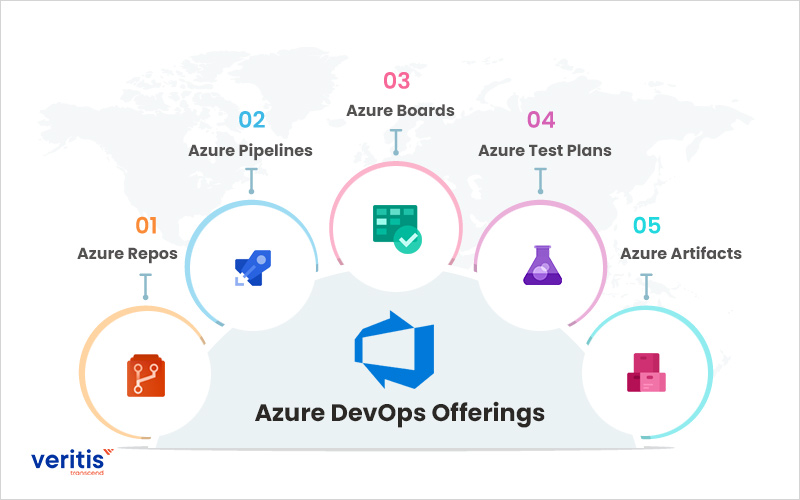
\includegraphics[width=0.5\columnwidth]{azure-devops-offerings.jpg}}
    \caption{Azure DevOps}
    \label{fig:Azure_DevOps}
\end{figure}

\textbf{Definition:} This platform acts as a comprehensive toolkit for software teams, offering various features to manage the entire development lifecycle efficiently.
\par
\textbf{Features:}
\begin{itemize}
    \item \textbf{Azure Repos:} This feature keeps your code organized and secure, just like a well-structured library holding all your project versions. It can use either Git or Team Foundation Version Control (TFVC) to manage your code.
    \item \textbf{Azure Pipelines:}  This service automates tasks like compiling code, running tests, and deploying new versions, saving time and minimizing errors.
    \item \textbf{Azure Boards:} Planning and tracking progress becomes transparent with this feature. It provides Kanban boards visually displaying tasks, backlogs listing upcoming work, and sprint planning tools.
    \item \textbf{Azure Artifacts:} Sharing reusable components becomes effortless with this feature. Think of it as a shared storage space for code modules, containerized applications, and other resources your team can easily access and reuse across projects.
\end{itemize}
\section*{Conclusion}
This chapter has comprehensively analyzed the current state of our cloud environment, infrastructure, and deployment process. We compared various cloud service models, ultimately selecting Microsoft Azure due to its alignment with our company's existing partnership and strategic goals. Within Azure, we identified Infrastructure as a Service (IaaS) and Platform as a Service (PaaS) as the most suitable offerings for our application's needs.
\par
Our in-depth examination of the existing infrastructure revealed a secure and well-structured architecture leveraging Azure's robust security features. Moving forward, we will delve deeper into Terraform and Azure DevOps, exploring their functionalities for enhanced infrastructure management and automated deployment processes. This comprehensive analysis establishes a solid foundation for transitioning to a secure, efficient, and automated cloud-based deployment framework.
